\section{Corrected results}
\label{sec:corrected}

\subsection{What was rebuilt}

The corrected vertex table carries the 1671 production triangle-filtered
rows unchanged, so it still serves the open-triangle consumers, and adds
the collapsed family $(1,\cos\gamma,\cos\gamma)$ sampled at the forty
plotted separations and refined between them. Three densities were built,
with 40, 79 and 157 collapsed nodes, by row selection from a single build,
which is exact because rows are independent.

Everything else is held at the deployed values: the same sixteen radial
shells, the same cosmology, the same tree-level bispectrum, the same
multipole cutoff of 1000, the same single quadrature window with 96
Gauss-Legendre nodes, and the same fold. Assembled on the deployed rows and
settings, the rebuild reproduces the deployed table to a median relative
difference of $3\times10^{-16}$ across all six channels, that is to
round-off. The difference between the deployed and corrected curves is
therefore the cosine sampling and nothing else.

\subsection{The grid density has converged}

Refining the collapsed family from 40 to 157 nodes leaves all four folded
observables \emph{bit-identical} (Figure~\ref{fig:resolution}). This is
stronger than convergence and it has a clean reason: once the queried
configurations are tabulated and the mesh key is fine enough to recognise
them, the callable returns the tabulated row directly and never consults
the refinement rows, so density beyond the queried set provably cannot
matter. With the production callable's coarser key the same comparison gave
differences of up to $4\times10^{-4}$, because thirty-eight of the forty
queries were failing the exact-match test and being interpolated
unnecessarily; Section~\ref{sec:callablefix} measures that.

The corrected curve is therefore a property of the vertex and not of the
mesh, in the strongest sense available: it is what the tabulated rows say.

\begin{figure}[t]
\centering
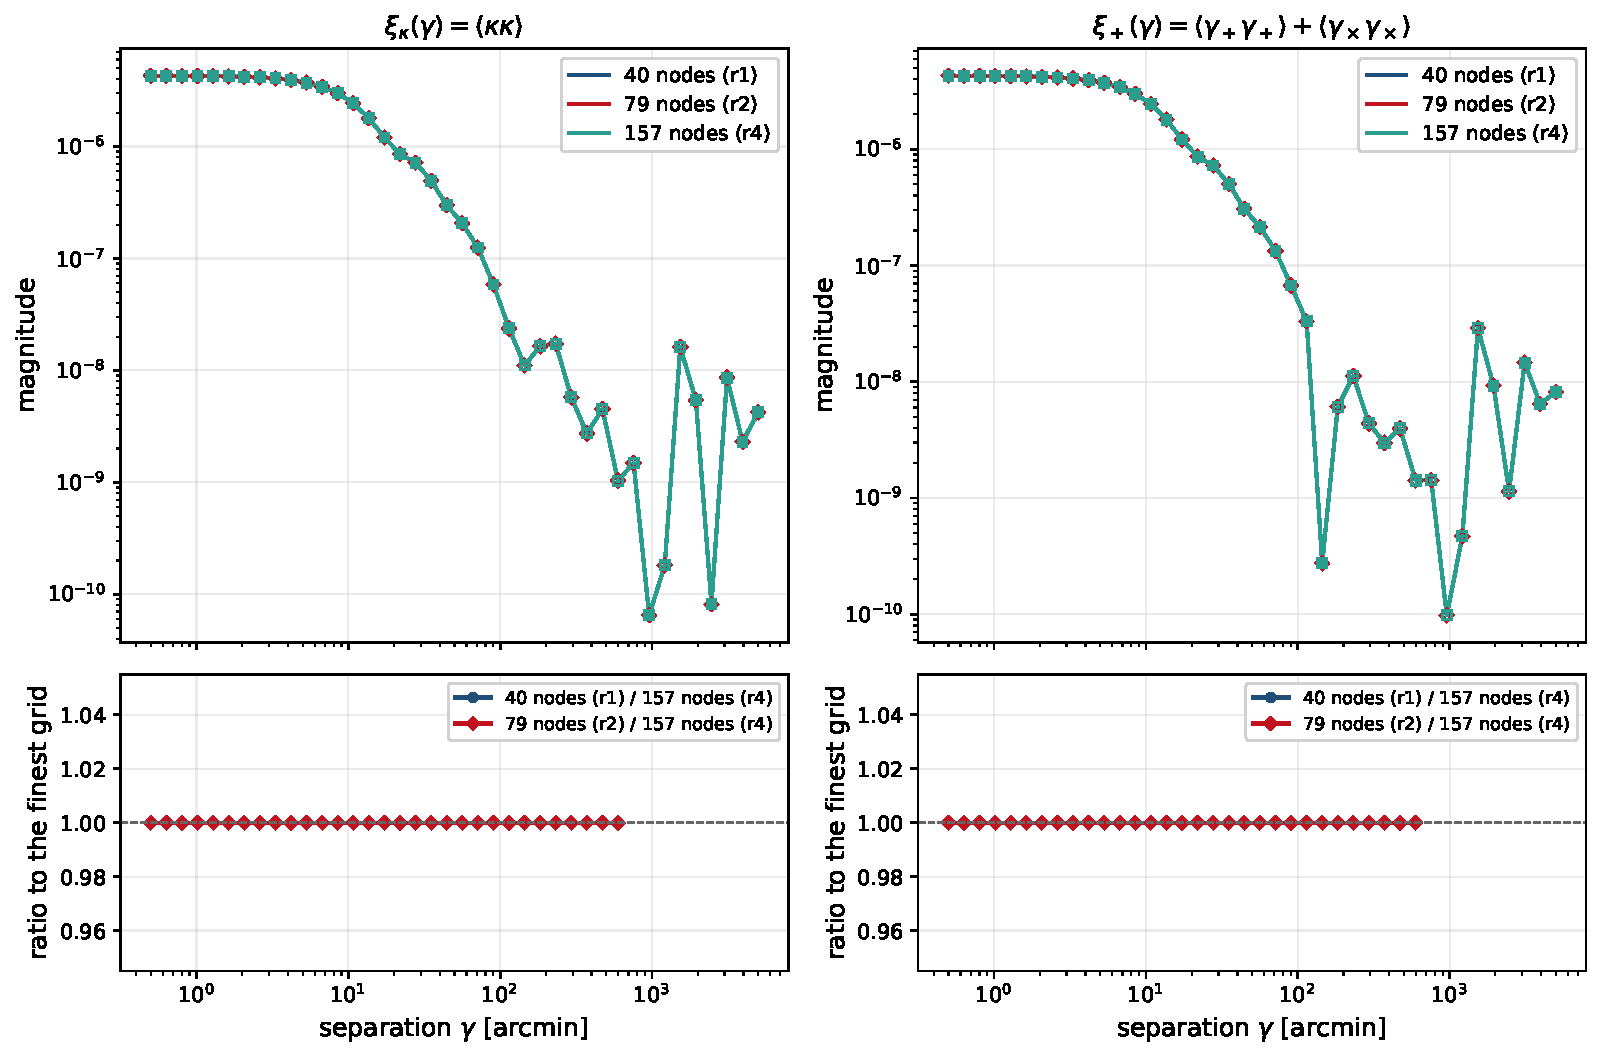
\includegraphics[width=\textwidth]{figures/grid_resolution.pdf}
\caption{Folded FK curves at three collapsed-grid densities, and their
ratios to the finest. The three agree to $4\times10^{-4}$. Produced by
\code{code/rebuild/fig\_convergence.py}.}
\label{fig:resolution}
\end{figure}

\subsection{The corrected two-point curves}

\begin{figure}[t]
\centering
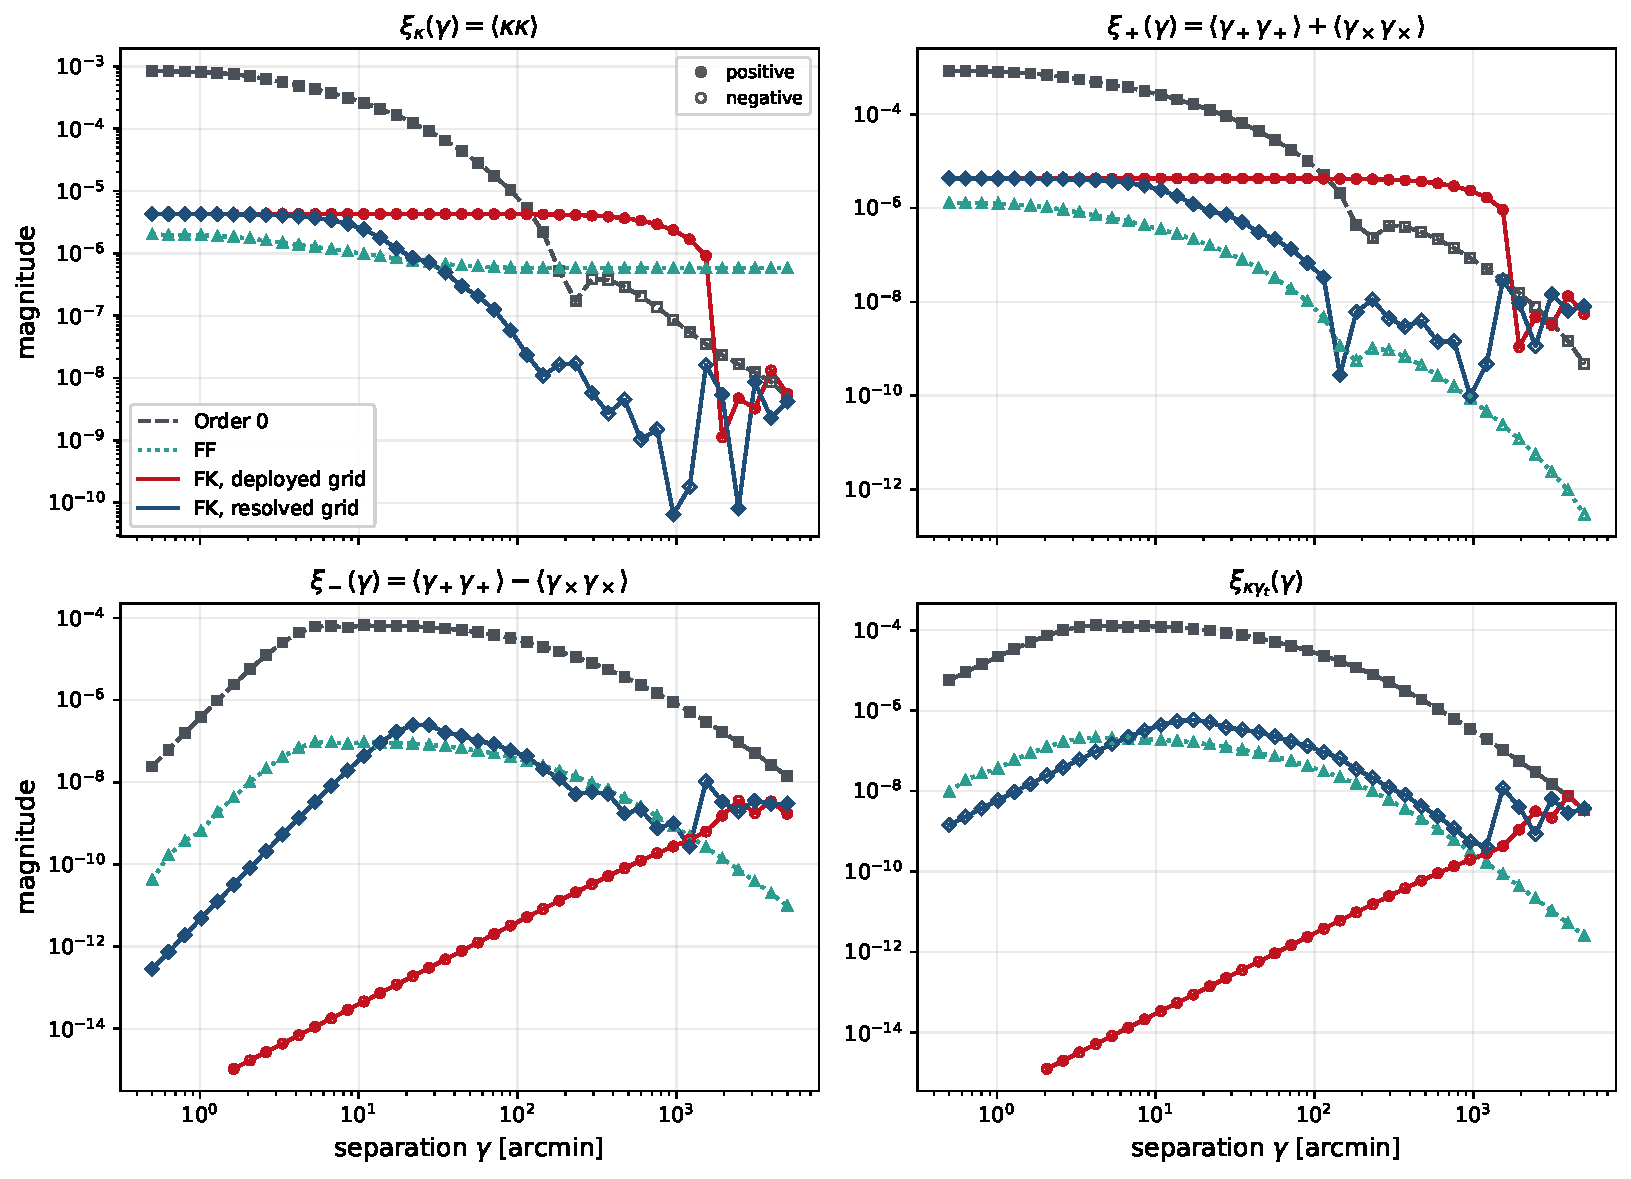
\includegraphics[width=\textwidth]{figures/grid_comparison.pdf}
\caption{The four plotted observables, with Order-0 and the Order-2 FF term
for scale. Red is the deployed FK curve, blue the same calculation with the
vertex sampled on the family it queries. Filled markers are positive,
open markers negative. Produced by
\code{code/rebuild/fig\_grid\_comparison.py}.}
\label{fig:grid}
\end{figure}

Table~\ref{tab:ratios} gives the numbers for $\xi_\kappa$.

\begin{table}[h]
\centering
\begin{tabular}{rrrrr}
\toprule
$\gamma$ [arcmin] & FK deployed & FK corrected & deployed/corrected & corrected/Order-0 \\
\midrule
   0.50 & $+4.2877\times10^{-6}$ & $+4.2815\times10^{-6}$ &     1.00 & 0.0051 \\
   5.30 & $+4.2876\times10^{-6}$ & $+3.7270\times10^{-6}$ &     1.15 & 0.0087 \\
   8.51 & $+4.2875\times10^{-6}$ & $+3.0037\times10^{-6}$ &     1.43 & 0.0096 \\
  21.88 & $+4.2863\times10^{-6}$ & $+8.7337\times10^{-7}$ &     4.91 & 0.0070 \\
  44.43 & $+4.2817\times10^{-6}$ & $+3.1491\times10^{-7}$ &    13.60 & 0.0071 \\
 114.27 & $+4.2483\times10^{-6}$ & $+4.2402\times10^{-8}$ &   100.19 & 0.0080 \\
 183.26 & $+4.1873\times10^{-6}$ & $+4.1908\times10^{-9}$ &   999.15 & 0.0081 \\
 232.08 & $+4.1282\times10^{-6}$ & $-5.1152\times10^{-9}$ & $-807$   & 0.0293 \\
 596.89 & $+3.3655\times10^{-6}$ & $-1.8661\times10^{-9}$ & $-1803$  & 0.0091 \\
\bottomrule
\end{tabular}
\caption{The FK contribution to $\xi_\kappa$ before and after resolving the
vertex, at fixed everything else. Beyond about $230'$ the corrected curve
has changed sign, so the ratio is negative and its magnitude is not
meaningful. Full table in \code{products/grid\_comparison\_table.txt}.}
\label{tab:ratios}
\end{table}

Three things change and one does not.

\paragraph{The arcminute amplitude survives.} At $\gamma=0.5'$ the
corrected value is $+4.2815\times10^{-6}$ against the published
$+4.2877\times10^{-6}$, a difference of $0.15\%$. The queried configuration
there really does sit on the tabulated corner, so the corner value is the
right answer. Every statement the draft makes about the arcminute
amplitude, including that FK is about twice FF there, stands.

\paragraph{The shape does not.} By $22'$ the published curve is too large
by a factor 4.9, by $114'$ by a factor 100, and beyond about $230'$ it has
the wrong sign as well.

\paragraph{There is no crossover.} At the deployed cutoff the corrected
FK/Order-0 ratio is between $0.5\%$ and $1\%$ at every separation that
carries signal. The two terms decay together. The published crossover near
$145'$ was the frozen corner value being compared against an Order-0 term
that genuinely decays. The ratio itself is cutoff dependent, rising to
between $1.4\%$ and $2.3\%$ at $\elmax=15360$
(Section~\ref{sec:cutoff}); what does not depend on the cutoff is that it
stays well below unity at every separation, so no crossover appears at any
cutoff tested.

\paragraph{The spin-2 observables are not empty.} With the vertex resolved,
$\xi_-$ reaches $+2.50\times10^{-7}$ near $28'$ and $\xi_{\kappa\gamma_t}$
reaches $-5.89\times10^{-7}$ near $17'$, about $0.4$ and $0.5\%$ of
Order-0, where the deployed run puts them at $10^{-16}$ to $10^{-9}$. The
exact cancellation the draft reports is a $\gamma\to0$ statement: at zero
separation $\zeta_{TPP}$, $\zeta_{PPP}$ and $\zeta_{TTP}$ vanish and the
$\xi_-$ combination cancels identically. It is not a statement about the
plotted range. These two values are quoted after the callable corrections
of Section~\ref{sec:callablefix}; without them they would read
$+2.86\times10^{-7}$ and $-8.88\times10^{-7}$.

\subsection{Harmonic space}

Transforming with the draft's own curved-sky Wigner-d kernels gives
Table~\ref{tab:cl}.

\begin{table}[h]
\centering
\begin{tabular}{rrrr}
\toprule
$\ell$ & $C_\ell^{\kappa\kappa}$, Order-0 & FK/Order-0, deployed & FK/Order-0, corrected \\
\midrule
   3 & $6.34\times10^{-8}$ & $+17.95$   & $-0.197$ \\
   5 & $7.97\times10^{-8}$ & $+9.02$    & $-0.002$ \\
   7 & $8.95\times10^{-8}$ & $+3.81$    & $+0.084$ \\
   9 & $9.75\times10^{-8}$ & $+0.87$    & $+0.034$ \\
  39 & $9.86\times10^{-8}$ & $+0.0008$  & $+0.0088$ \\
 115 & $4.61\times10^{-8}$ & $-0.0012$  & $+0.0079$ \\
 415 & $8.33\times10^{-9}$ & $-0.0001$  & $+0.0091$ \\
 789 & $2.52\times10^{-9}$ & $-0.0001$  & $+0.0089$ \\
\bottomrule
\end{tabular}
\caption{FK relative to Order-0 in $C_\ell^{\kappa\kappa}$, using the
generator's own transform. The factor 18 excess at $\ell=3$ is the
sampling artefact. The corrected FK is a steady $0.8$ to $0.9\%$ correction
over $39\le\ell\le800$; the residuals at $\ell<10$ are of order 10 to 20
percent and are within the finite-range and apodisation systematics the
generator documents. Produced by \code{code/rebuild/cl\_ratio.py}.}
\label{tab:cl}
\end{table}
